\documentclass[conference]{IEEEtran}
\IEEEoverridecommandlockouts
% The preceding line is only needed to identify funding in the first footnote. If that is unneeded, please comment it out.
\usepackage{cite}
\usepackage{amsmath,amssymb,amsfonts}
\usepackage{algorithm,algorithmic}
\usepackage{graphicx}
\usepackage{listings}
\usepackage{textcomp}
\usepackage{xcolor}
\def\BibTeX{{\rm B\kern-.05em{\sc i\kern-.025em b}\kern-.08em
    T\kern-.1667em\lower.7ex\hbox{E}\kern-.125emX}}
\definecolor{lightgray}{rgb}{.9,.9,.9}
\definecolor{darkgray}{rgb}{.4,.4,.4}
\definecolor{purple}{rgb}{0.65, 0.12, 0.82}

\lstdefinelanguage{JavaScript}{
  keywords={typeof, new, true, false, catch, function, return, null, catch, switch, var, if, in, while, do, else, case, break},
  keywordstyle=\color{blue}\bfseries,
  ndkeywords={class, export, boolean, throw, implements, import, this},
  ndkeywordstyle=\color{darkgray}\bfseries,
  identifierstyle=\color{black},
  sensitive=false,
  comment=[l]{//},
  morecomment=[s]{/*}{*/},
  commentstyle=\color{purple}\ttfamily,
  stringstyle=\color{red}\ttfamily,
  morestring=[b]',
  morestring=[b]"
}

\lstset{
   language=JavaScript,
   backgroundcolor=\color{lightgray},
   extendedchars=true,
   % frame=single,
   basicstyle=\small\ttfamily,
   showstringspaces=false,
   showspaces=false,
   tabsize=2,
   breaklines=true,
   showtabs=false,
   captionpos=b
}
\begin{document}

\title{User Interface for Video and Image Stitching}

\author{
\IEEEauthorblockN{1\textsuperscript{st} Nguyen, Trung Han}
\IEEEauthorblockA{\textit{Open Distributed Systems} \\
\textit{Technische Universität Berlin}\\
Berlin, Germnay \\
trung.h.nguyen@campus.tu-berlin.de
}
\and
\IEEEauthorblockN{2\textsuperscript{nd} Tran, Minh Duc}
\IEEEauthorblockA{\textit{Open Distributed Systems} \\
\textit{Technische Universität Berlin}\\
Berlin, Germnay \\
minh.d.tran@campus.tu-berlin.de
}
\and
\IEEEauthorblockN{3\textsuperscript{rd} Tran, Nhat Duc}
\IEEEauthorblockA{\textit{Open Distributed Systems} \\
\textit{Technische Universität Berlin}\\
Berlin, Germnay \\
nhat.d.tran@campus.tu-berlin.de
}
}

\maketitle

\begin{abstract}
This document is a model and instructions for \LaTeX.
This and the IEEEtran.cls file define the components of your paper [title, text, heads, etc.]. *CRITICAL: Do Not Use Symbols, Special Characters, Footnotes, 
or Math in Paper Title or Abstract.
\end{abstract}

\begin{IEEEkeywords}
web UI, video and image stitching, MPD, DASH, Amazon Simple Queue Service (SQS)
\end{IEEEkeywords}

\section{Introduction}
With the recent progresses in cloud computing in the areas of cost-efficiency, scalability etc., more and more software applications are shifted from local computers to external servers.
While in the past software like audio or graphics editor tools had to be installed locally due to high processing demands, nowadays mentioned applications can be provided over the internet.

The Fraunhofer FOKUS\footnote{https://www.fokus.fraunhofer.de/} \textit{(Fraunhofer Institute for Open Communication Systems)} is a research unit of the Fraunhofer Society\footnote{https://www.fraunhofer.de/} and is concerned with applied research and development of applications in the field of Information and Communications Technology.
Among the projects of FOKUS is the development of such a service for video and image stitching, similar to well-known traditional software like Window's Movie Maker\footnote{http://windows.microsoft.com/en-us/windows/get-movie-maker-download}, but in this case over the internet.

Using media URLs from any host or cloud provider, the backend creates an MPD file (manifest file for adaptive media streaming\cite{Sodagar}) according to a given stitching configuration.
Amazon's Simple Queue Service\footnote{http://aws.amazon.com/sqs/} (SQS) serves as communication channel between frontend and service backend.

As of now FOKUS has only implemented a stitching backend. A proper user interface for seamless interaction with the backend is still missing.
In this work we implemented a web UI\footnote{Code available at https://github.com/SmokyDesperado/moveditor} for that very purpose.

In particular this inlcudes:
\textbf{(II)} A glimpse into related work and what elevates this work.
\textbf{(III)} and \textbf{(IV)} The Architecture and implementation, in which non-trivial steps are described and important decisions made while developing the UI are explained.
\textbf{(V)} An evaluation of the approach taken for implementing the user interface as well as a discussion of its strong points but also its flaws.
\textbf{(VI)} A conclusion to this work and suggestions for future work.

\section{Related Work}
%List online/offline video stitching tools, differences and what makes our web app unique...
There are various programs avaiabale to edit videos, images and audios into one file.
The majority of them are video editing tools.

For example, Mircosoft Fotos \footnote{https://www.microsoft.com/de-de/p/microsoft-fotos/9wzdncrfjbh4}, the successor of Windows Movie Maker and one of the plainest video editing tools, is able to stitch videos, images and audios.
This software can not overlap video and picture track with soundtrack.

Adobe Premiere Pro \footnote{https://www.adobe.com/products/premiere.html} is the industry-leading video editing software. 
It also supports the functions to adjust the length of different media files as well as stitch them together. 
It is not possible to export a Adobe Premiere Pro project as a dash file.

An online solution for video editing is Movie Maker Online\footnote{http://moviemakeronline.com/}. 
This Editor has every editing functionalities that we need but it also do not support to export as a dash file.

\section{Architecture \& Used Technologies}
%Web UI communicates with FH backend via SQS; using AngularJS, AWS SDK, clouds...
The architecture we used is similar to the classic back-end architecture.
We have a front-end that is executed on the client side.
The JavaScript, HTML and CSS code runs in the user's browser and creates the user interface as a web app.
Users edit video, image and audio files and finish their work by sending segmentation and stitching requests to the back-end.
Frauenhofer FOKUS provides the back-end.
The code of the back-end runs on an Amazon server.
It receives receives segmentation and stitching requests from the web app and replies with MPD URLs.

Our web app uses the AngularJS framework.
Video, image and audio files have to be stored online, for example cloud storage like Google Drive, Dropbox or even YouTube.
In order to access these media files in the app, the file URLs have to be public to ensure that the app can load the files.

The front-end communicates with the back-end via SQS by using AWS SDK \textit{(Amazon Web Services Software Development Kit)}.
Every client side request will be pushed on the request queue.
The back-end notices the request, processes the request and replies by pushing the result on the result queue.
Results on the result queue will be processed by each listening client.

\textbf{ToDO Han, diagramm von Cloud, Web App und Frauenhofer fokus}

\section{Design \& Implementation}
List some features etc. but this section will only focus on main aspects of our web ui implementation and why things were done that way, bower (what?, why?, how?) + setup, ...

This section will focus on the realisation of the project, what was done and the reasons behind. It will give a better view on the main implementation aspects of the app and not providing a detailed documentation about every single part.

\subsection{General}
The implementation of the app used various libraries. The main structure of is based on the AngularJS project scaffolding by Yeoman\footnote{http://yeoman.io/learning/}. This provide a ready to use AngularJS project, with directory structure, default templates and installs required components and components to boost the development process. 

Node.js\footnote{https://nodejs.org/en/} is the main run-time enviroment for the development process and is used to create the server while developing. New modules to help the development can be installed via the package manager npm\footnote{https://www.npmjs.com/}. The used packages are saved in the file package.json and can be manage there, like changing the used package or the package version.

Grunt\footnote{https://gruntjs.com/}, a task node runner module, is used for the actual development server configuration. It gives the possibility to define tasks and used them to creates custom development conditions and helper. Task can be defined in the required Gruntfile. While the predefined task serve a local server on port 9000 with live reload creates, will build concat, minify, uglify and do some other optimisation to the code and output it in a specified directory. This task is used for production deployment.

For client sided libraries the Node module Bower\footnote{https://bower.io/} is used. Like the Node file package.json bower has it own package management file bower.json. There the used libraries for the app are listed and can be managed easily. 

AngularJs is used as the main JavaScript framework and allows the implementation of single page application to create a native app like user experience. Furthermore the provided functionalities of AngularJS like ng-if, ng-repeat, ng-class attributes in the HTML template files and the two-way-binding (AngularJS handles the synchronisation of specified variables) reduce the manual binding between HTML and JavaScript files. The ability to creates reuseable modules, called directives, gives a big impact in reducing duplicated codes and improves the code management.

\subsection{Content}
The content area contains all the base videos, images and audios which are used in the app to stitch and create a new video. It is devided into two segments, the menu at the top and below the actual content area with all the materials. New content materials are loaded and added to the area by a public accessible URL. Meta information, like the thumbnail or content length, will be loaded and added to visible representation of the material. Content materials can be dragged and moved around to add them in the timeline or delete them. The user also has the possibility to save and load the current session and watch or hear the content material if the content of the material is unknown or forgotten.

For displaying the materials in the content area the contentList object is used and binded to the view. This object is a simple JavaScript dictionary object which consist of a random generated contentId as key and an instance of the JavaScript class Content as value. The dictionary data type was chosen to eneabled the possibility of having direct access to the object of the contentList by only knowing the contentId. It is possible to pass the contentId of the materias from one service to another and only access the needed material properties right before using.

The instances of the Content class consist of a name, a type, a length, a url, a mpd and a active property. The name property is empty at the beginning and a user can change the name after the content materia is loaded. The url property is is the public accessible URL of the video, audio or image which is used to add the material. It is not possible to changed it afterwards. Each material URL is unique for the contentList. Dublicated material URLs will not be added to the contentList. As a result that only the URL is validated and not the content of the material, a duplicated content material can be added to the list by using the same content but with different URLs. New content is added to the contentList by adding a video, image or audio to a cloud or web service with a public accessible URL and the adding this url to the input field of the content area menu.\\
\\
== bild vom content material ==\\
\\
The meta information of the content material, like type and the length, are loaded after adding the content to the list by the HTML Audio/Video Events. For a better visualisation an image of the middle of the material video is added as a thmubnail while loading the meta information. The image itself is used for image typed content and for audio typed materials a pre defined image is used. Farther an icon on the lower right corner of the content also indicates the typed of the content material.

The active property of a material is used to keep track of amounts of the material used in the timeline. Each material adding to the timeline increase the active counter and each remove from the timeline decrease the counter. Unless the active property equals 0 it is not possible to delete the content material. The last property the mpd property is not editable by the user. It is used to store the mpd URL after the segmentation process of the backend and then used for the stitching request.

The drag and drop functionality to add content materials into the timeline or delete content is enabled through the AngularJS module AngularHammer\footnote{https://github.com/RyanMullins/angular-hammer} by Ryan Mullins. The already existing touch, mouse and pointerEvents recognition JavaScript library HAMMER.JS\footnote{http://hammerjs.github.io/getting-started} was made into a AngularJS module for a simple usage. The three important features of this module were the panStart, panMove and panEnd events. PanMove provided functionalites to recognise the mouse events and manipulate the DOM element while panStart and panEnd provided manupulation right before and after panMove is executed. So it was possible to initialise needed helper variables (i.e. activate attributes to react while moving) or saving the current app state after moving elements. Dragging materials will create a drag indicator, showing and representing the active drag action. The indicator will disappear by dropping the material (mousekey up) and execute the specific action depending on the dropping mouse position.

A trash icon is start to appear in the content area by dragging a material element around. When the user drops it in the trash and the mouse position is within the boundaries of the trash icon, then this action will remove the material from the content area (when active is 0). Showing and hiding the trash is activated by panStart and panEnd. Dropping the material into the timeline will add a chunk in the timeline area.

Another aspect of the content area menu is saving and loading working sessions. Saving can save the current state of the content and timeline area and loading wiill recreate the state of a saved working session from a file. Based on the used data structure of the app, the saving file is a .txt file containing one JSON object. The save process will collect all needed information of the different parts and create the saving file and loading will read the file and recreates saved state of the app. Because of the simplicity of the saved file and the absent of validation while loading, a use can manupulate the information and the state of the app.

For checking the loaded content, the user can double click on the specific material. This opens up a pop up viewer / player showing image typed materials or playing video or audio typed materials. The double click is handled by AngularHammer and will create an overlay on the app. Normally the overlay is hided in the background and jumps to the foreground when activated. The dynamically created and added content of the overlay depends on the type, whether it is a audio player, a video player or just a image, of the material. By clicking outside the overlay content, the content will be pause (only for audio and video player), destroyed and the overlay will hide in the background again.\\
\\

\subsection{Timeline Area}
Mainly the user will be working in the timeline area to create and edit the stitching video. Unlike the content area, the timeline area is devieded into three segments, the timeline bar where the materials are added as chunks, a menu to execute serveral functionalities and an information area to view the chunk data. Added chunks of the timeline can be focused and edited by dragging or by interaction with the menu buttons. The information area will show meta more detailed information of focused chunks.

Chunks are JavaScript objects with data about how the material is used in the timeline. The properties of chunks are objectListId, start, end, offset, mute and name. Naming chunks should help the user to easily distinguishing two different chunks of the same material. Names of chunks are the same from the created material and can be changed afterwards by the user. Mute allowes the user to turn of the sounds of a video or audio while playpack. The properties start and end are the time values when it starts and when it ends in the timeline. Offset indicates after which time of the original material the chunk starts to play, like if the user wants to start from the middle of the material. To connect between the chunks of the timeline and the material of the content, the objectListId is used. It has the contentId of the material and is used to get the originated material properties (length, url, type etc.) of the chunks, to avoid duplicated data in the chunks.

Added material chunks in the timeline are stored in a array, called timelineList, unlike the contentList dictionary object. Reason for that is to have a simple way to store the material chunks and having a ordered data structure. The amount of same chunks in the timeline is unlimited. Like the contentList object, the elements of the timelineList is used to generate a visual representation of the chunks. Due to the characteristic of overlap between video and audio content, the timeline is devided into two parts. Video and image chunks (no overlapping allowed) are positioned in one timeline part and audio chunks are positioned on a seperate timeline part and can be played at the same time like the video / image chunks.

The scaling on the timeline makes it easier to estimate the start and end position of chunks. This scaling is dynamically created depending to the total length of the created video content. An important variable to this aspect is the pixelPerSeconds value, on which the dynamic calculations are based on. Mainly it is used to calculate the pixel position of the mouse or chunks on the timeline to a timevalue and vice versa, because the drag events are working with pixel values, but the chunks requires time values. The visible timeline scales are basicly dynamic created DOM block elements, which positioned is calculated then by the pixelPerSeconds and the time amount of the scale step size. The menu buttons for zooming changes the pixelPerSeconds and the scale steps value and the two way binding mechanism of AngularJS updated the visual of the timeline according to the values.

Most of the chunk editing functionalities are chunks specific, so the chunks in the timeline can be focused by click (AngularHammer event used). A second click on the same and a click on another chunk will end the focus. A required focus for chunk editing is the deleting button. The click on this menu button only deletes the focused chunks, by removing the element from the array and does nothing, if no chunk is focused.

To rearange the time position of the chunks in the timeline, the user can drag the chunks and move them in the timeline. Like in the content area, this dragging feature is provided by AngularHammer. To only allow the chunks to move in a limited range, like the start and end of timeline or end of previous chunk and start of next chunk, the panStart event calculate this values before the panMove event. In the first version, the limits were used to check if panMove is allowed or not. Due to the delayed detection of fast mouse movement postions, the dragging was often stops right before the limited position and a space was presented in between. The optimization afterwards used the limits to detect of the chunk positon if within the allowd space and set it to the limit value, if these boundaries are exceeded. The panEnd event then calculates the pixel positon of the chunks to a time value and set them. To reduce the required mouse position precision by the user, the time value calculations will be quantized by 100 ms. This may reduce contents, but the chance of users recognising the difference is small and acceptable.

Like dragging the chunks within the free given space of the timeline, the shortening of the start and the end of chunks is executed by dragging the chunk modifier. These modifier are visible when the chunk is focused and not dragged. The limits for the modifier are, besides the limits of the chunk dragging limits, when the original start and end of the material. This additional limits prevents chunk offsets less than 0 and ends greater then length of the material. 

Originally it was planed to move chunks in the timeline and reordering the chunks by dragging them. To avoid accidential reordering while moving chunks and increase the UX, the reordering was lastly implemented by menu action buttons. Focused chunks can swapped the order with the previous or the next chunks, by reordering the element position within the timelineList array. 

Another timeline editing feature requiring chunk focus is the chunk cutting. This allows the user to cut one chunk by the specified time position into two seperate chunks, one ends and one starts by the cutted position. A modified chunk clone will be added in the timelineList after the the position of the cutted chunk. The clone and the cutted chunk values are then setted new. The chunk start of the cutted and the chunk end of the cloned chunks remain the same. The chunk end of the cutted and the chunk start of the cloned are set to the quantized cutting position. The offset of the clone musst then recalculated by the origingal offset adding the difference by the cut. 

If the user make a wrong actions in the timeline, the undo button in the menu helps them to jump back in the execution of timeline actions. There are ten chronologically ordered states of the timeline stored in the savedSteps array. The states are JSON converted string of the timelineList pushed into savedSteps after certain (panEnd, swap etc.) timeline action. The JSON string convertion is needen, because by adding only the timelineList into the array will only reference to the timelineList. So each added state reference to the timelineList and will not contain the chronological state changes but the current state of timelineList. To keep savedSteps to ten states, adding a eleventh state will remove the first state of the array. Undo allows the user to jump back up to ten steps and the redo button will jump foreward up to the current state. The savedStepPointer tracks the current position in the chronological array while moving for- and backward. \\

\subsection{Preview Player}
The preview player emulates the stitching result of the service backend without actually sending the necessary requests.
In doing so, imperfections in the stitching configurations can be detected and corrected via real-time feedback.
Users are not impelled to wait for the actual stitching response, thus saving them time.
\begin{figure}[H]
\centering
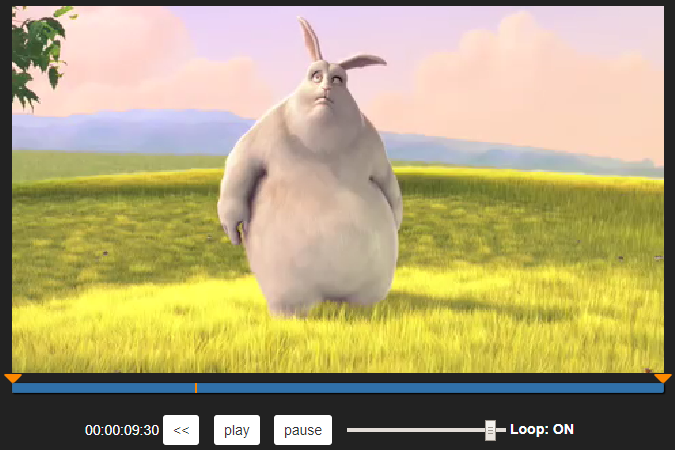
\includegraphics[scale=0.5]{preview_player.png}
\caption{UI of Preview Player.}
\end{figure}
\subsubsection{Preview Player - Features}
The implemented preview player supports all common controls of a usual browser media player.
These include: a ``play/pause''-button, a ``time-position''-slider and a ``volume''-slider.
On top of that, a ``restart''-button, a ``loop-play''-toggle and a ``play-in-range''-slider were added.
For the latter the \textit{noUiSlider}\footnote{https://refreshless.com/nouislider/} library is utilized.
Functionally, the ``play-in-range''-slider marks a time range in which the ``time-position''-slider is contraint.
Almost all of the listed controls can be operated via shortkeys\footnote{manual/wiki} making the web UI feel more like a native application.
\\
\subsubsection{Preview Playback - Logic}
For audio and image preview playback it is sufficient to only have one HTML audio, respectively image, element and change its sources in real-time while playing.
However, this method does not work for all video sources, e.g. cloud provider URLs generally take more time for the initial loading which leads to stuttering, especially right after swapping video sources.
Therefore, per video chunk the implemented player creates one dedicated HTML video element with preloaded source.
While playing, it then only manipulates the z-indexes of the video elements and stops or starts them accordingly (see Algorithm 1) resulting in a smoother playback and minimized buffering time.

As optimization, whenever a new video chunk is added to the timeline area, the preview player is signalled to inspect whether there already exists an HTML video element referencing the same source.
If there is none, then one will be created.
Analogously, if a video chunk is removed from the timeline, then its corresponding HTML video element is deleted if there is no other chunk requiring the same source.
\begin{algorithm}[H]
\caption{Preview playback loop, simplified}
	\begin{algorithmic}[1]
		\STATE cc $\gets$ current chunk
		\STATE pc $\gets$ previous chunk
		\IF {cc $\ne$ pc $\AND$ (pc.type $=$ video $\OR$ pc.type $=$ audio)}
		\STATE pcHTML $\gets$ corresponding HTML video/audio element
		\STATE pause pcHTML
		\ENDIF
		\IF {time $=$ timeline-end $\OR$ time $=$ range-end}
		\IF {loop play active}
		\STATE go to range-start
		\ELSE
		\STATE pause player
		\RETURN
		\ENDIF
		\ENDIF
		\STATE bring current video/image to the front via z-index
		\IF {cc.type $=$ video $\OR$ cc.type $=$ audio}
		\STATE ccHTML $\gets$ corresponding HTML video/audio element
		\STATE calculate ccHTML offset position
		\STATE mute ccHTML if necessary
		\STATE play ccHTML
		\ENDIF
		\STATE pc $\gets$ cc
		\STATE time $\gets$ time counter + 100 ms
		\STATE diff $\gets$ (real-time-passed - time)
		\STATE repeat Algorithm 1 in (100 ms - diff)
	\end{algorithmic}
\end{algorithm}
Due to the nature of Javascript, Algorithm 1 had to be seperated into two functions code-wise or else the parallel updated time counter would start one loop ahead of the preview player resulting in both units not being in sync.
To keep the time counter even more precise, a self-adjustment calculation was introduced. By tracking the real-world time passed and matching that with the internal player time, it can be ensured that the preview playback loop is almost always repeated accurately every 100 milliseconds.

\subsection{SQS}
Once the user is satisfied with the constructed timeline chunks, the whole stitching procedure can be initiated by pressing the ``stitching''-button.
The stitching process consists of two phases: 1.) A segmentation phase and 2.) a stitching phase.

For communicating, the stitching backend operates over two seperate SQS queues.
From the web client perspective, one queue is for sending requests, the other is needed for receiving results.
Both are used for segmentation as well as for stitching requests.
The request type is determined through the message body by the service backend.
Further, each message body possesses a user defined \textit{jobID} which helps users to identify their messages in the queue for responses.
As with other libraries utilized in the developed user interface, functionalities of Amazon's SQS were made accessible by incorporating the official AWS SDK\footnote{https://github.com/aws/aws-sdk-js\#using-bower} for JavaScript via Bower.
\begin{figure}[H]
\begin{lstlisting}
var sqs = new AWS.SQS({
  "accessKeyId": sqsAccessKeyId,
  "secretAccessKey": sqsSecretAccessKey,
  "region": sqsRegion
});
\end{lstlisting}
\caption{Setting up an SQS instance in AngularJS.}
\end{figure}
At the beginning, the condition of the timeline and content area at process starting time are temporarily preserved.
By working on those data, accidental user changes and edits in the meantime don't affect the stitching procedure.
To avoid further problems, it is not possible to send another stitching request until the whole process is completed.
\\
\subsubsection{Segmentation Phase}
In this context, segmentation means creating an MPD file based on an audio, image or video file, requiring only a publicly accessible resource URL.
Theoretically, since fragmentation is applied to files in full length and not single chunks, this step could be executed as soon as a source is added to the content area or when a content is added to the timeline.
However, the user has to wait for the stitching process either way and not every resource might be used in the end which would then lead to spamming and wasting storage of the FOKUS backend.
Also worth mentioning is that for segmenting images a length must be specified priorly which is only possible after actually working on the timeline.

During phase 1, chunks in the timeline are fragmented in chronological order.
A segmentation request message to a chunk is created and put on the request queue (see Fig. 2). While images need an extra \textit{loop} attribute compared to videos to indicate their length, audio files require an \textit{onlyaudio} attribute, although the fragmentation of latter are currently not supported by the backend.
\begin{figure}[H]
\begin{lstlisting}
var msg = {
  jobID: segmentationId,
  S3URL: chunkUrl,
  encodingprofile: "default",
  requestEnqueueTime: +new Date()
};

var params = {
  MessageBody: JSON.stringify(msg),
  QueueUrl: requestQueueURL,
  MessageGroupId: 'myGroupId'
};

sqs.sendMessage(params, function(err, data) {
  if (err) {
    console.log('ERROR: ', err);
  } else {
    console.log("send request successfully");
  }
});
\end{lstlisting}
\caption{Example request for segmenting a video.}
\end{figure}
After the segmentation request was send, the result queue will be polled for via a recursive receiving function.
The reason for this lies in the AWS SDK, which only allows the client to receive at most the 10 oldest messages on the result queue.
This in turn means that if 10 or more messages of other users are occupying the queue first, then the client has to wait until those are removed by their target user. 

The implemented approach polls for the maximum number of 10 messages at a time and only considers those targeting the user via identifying the \textit{jobID}.
Are among those messages no result messages, a progress per chunk fragmentation is shown and the next 10 are polled for.
In case one segmentation is done, a message contains an MPD URL, which is saved temporarily and the next chunk will be segmented, but only if its corresponding source URL has not been segmented yet.
Either way, those messages are then removed from the queue by its proper recipient so that the next responses in the FIFO queue can be received.

By default, short polling is used in SQS.
Long polling though yields several benefits and is enabled by setting the \textit{WaitTimeSeconds} parameter when receiving messages from a queue.
The developed algorithm uses the maximum value of 20 seconds.
This way, the probability of getting empty replies is disposed of by waiting until messages are available before responding to the client.
Nevertheless, messages are still returned as soon as they become obtainable.
Long polling further queries all Amazon SQS servers instead of a mere subset so that false empty responses are avoided, too.
\\
\subsubsection{Stitching Phase}
Are all chunks segmented successfully, the stitching phase starts.
By sewing MPDs together according to a specified configuration, a new video MPD is generated.
Except the message to be transmitted, sending and receiving a stitching request are analog to that of a segmentation request.
\begin{figure}[H]
\begin{lstlisting}
var configStitching = {
  "LOG_LEVEL": "info",
  "server": {
    "url": "http://localhost:8090",
    "staticFolder": "adstitcher-srv/public/mpds",
    "dashEndpoint": "/Users/fr/Documents/adstitcher-srv/public/mpds/"
  },
  "content": [
    {
      "type":"video",
      "begin":0.8,
      "end":5.5,
      "offset":0,
      "mute":false,
      "hide":false,
      "url":"https://s3.eu-central-1.amazonaws.com/wesualizesegment/exampleVideo1/Manifest.mpd"
    },
    {
      "type":"video",
      "begin":6.3,
      "end":10.0,
      "offset":3.7,
      "mute":false,
      "hide":false,
      "url":"https://s3.eu-central-1.amazonaws.com/wesualizesegment/exampleVideo2/Manifest.mpd"
    }
  ]
}

var msg = {
  jobID: stitchingId,
  config: configStitching,
  requestEnqueueTime: +new Date()
};
\end{lstlisting}
\caption{Example message of a stitching request}
\end{figure}
While the segmentation works perfectly, the stitching request results in an error (\textit{errorCode 11: "something wrong with the dashEndpoint in the config. Please check the input config."}).
Since the \textit{dashEndpoint} information was provided to us and there was no documentation of the stitching backend as well as the developers not always being contactable, this issue could not be resolved in this work.
\\
\subsubsection{Problems when receiving messages}
During tests it became apparent, that not every polling call resulted in the client receiving messages.
Despite that, when only one client is polling for the FIFO result queue at a time, it works perfectly.
As soon as more users attempt to receive messages, the whole process is slowed down massively even though long polling is used.
It may be that the concurrent pollings from different clients are interferring with each other so that the probability of not receiving any messages is increased greatly.
This way, the FIFO queue can not make any or only very slow progresses.
On the other hand it might also be that the SQS queues are deployed on budget servers that are not able to actually handle multiple requests simultaneously.

Even worse, when many clients are polling for results, and some of these abort this process, then that might lead to stagnation of the result queue, whereby no active user can receive any more messages.

In this prototype version of the UI, a ``purge\&restart''-button was implemented as a safety measure for now.
This button will remove all messages on the queue and restart the FOKUS backend server, although this is no longterm solution to menttioned problems.

\section{Discussion}
What works, what does not? Shortcoming?\\

- SQS and FH backend are shit; a intermediary backend managing the request (msg timeouts etc...) and providing an API would be better; suitability for use with regard to user-friendliness, performance, robustness... \\
- server und queues nicht robust \\
Shortcomings: quantization 100ms -$>$ video ende abgeschnitten, 10ms -$>$ schwächere cpu schaffen nicht\\

\section{Conclusion}
In this work a prototype of a user interface offering many features and options for video and image stitching was implemented.
Video, audio and image content resources can be added to the application by simply using a publicly accessible URL.
On a timeline, chunks can be constructed to a new video by utilizing different editing possibilities.
Real-time feedback is given via a dedicated preview player emulating the stitching results without doing actual video cutting or processing.
By serializing whole working sessions, its state can be shared or recalled conveniently at a later time.
One of the main purposes however, i.e. to make the UI interact with the existing stitching backend by Fraunhofer FOKUS, could be satisfied only partially.
Having one sole client communicate with the provided FIFO queues is working perfectly fine.
As soon as more users concurrently attempt to poll for answers on the result queue, that queue becomes a bottleneck even though a more beneficial long polling method is used.
The reason for that might be in the implemented receiving algorithm or in the load handling capability of the server deploying the queues.
Possible solutions involve approaches using an intermediary backend to take care of sending and receiving messages from the SQS queues.
Another issue we encountered is that while the segmentation phase delivers the expected MPDs, the stitching phase results in an error.
Since there was no documentation of the FOKUS backend and with its developers not always being contactable, this problem could not be resolved in our work as of now.
In spite of mentioned deficiencies, the implemented prototype still qualifies as a fully functional user interface and forms the basis for the frontend of the existing stitching backend by Fraunhofer FOKUS.

\subsubsection*{Future Work}
While the realized prototype provides many user interaction possibilities, there is still room for further valuable features and improvements.
One of the most handy additions would be to control the preview player time and play-in-range positions by utilizing the currently only indicating position markers on the timeline.
Also, the un-/redo features merely apply for timeline changes at the moment.
When executed, ``active-element''-updates on content resources through adding and deleting chunks won't be taken into account.
It is desired to monitor these changes and other operations done on the content area.
Furthermore, dragging new chunks to the timeline, moving or shortening chunks would be more appealing if tooltips are displayed which show time stamps during these actions to increase the user experience.
Although adding of new content resources works, the URL acceptance check and resource type whitelist matching algorithms would benefit from enhancements, too.
Loading saved session files might need correctness checks in a future revision as well, so that this point can not be exploited, providing more robustness and consistency.

Regarding the communication with SQS, besides fixing the stitching phase error, it is suggested to implement a dedicated intermediary backend to take care of sending and receiving messages (as mentioned in \textbf{V. Discussion}).
Otherwise, strategies must be devised, so that concurrently receiving clients won't result in a bottleneck.

\begin{thebibliography}{00}
\bibitem{Sodagar} I. Sodagar, ``The MPEG-DASH Standard for Multimedia Streaming Over the Internet'', in IEEE MultiMedia, vol. 18, no. 4, pp. 62-67, Washington, D.C.: IEEE Computer Society, October 2011. doi:10.1109/MMUL.2011.71
\end{thebibliography}

\end{document}
